%Autor: miguev

\chapter{\LyX}

La mayor�a de los procesadores de textos est�n basados en la filosof�a
WYSIWYG (what you see is what you get, lo que ves es lo que tienes) en
la que el usuario no s�lo  tiene que escribir sino tambi�n preocuparse
de d�nde aparacer�  cada elemento en el documento final.  Esto lleva a
conservar pr�cticas antiguas provenientes  de las m�quinas de escribir
mec�nicas. Entre  estas pr�cticas  todos conocen los  tabuladores, los
guiones para partir palabras al final de l�nea, dejar varias l�neas en
blanco para rellenar, etc. Todo eso es definitivamente prediluviano.

\LyX, a diferencia  de los dem�s procesadores de texto,  es lo que se
denomina un  programa WYSIWYM (what you  see is what you  mean, lo que
ves es lo que quieres decir).  Esta filosof�a de hacer un documento se
basa  en que  el usuario  no debe  preocuparse de  la composici�n  del
texto, sino �nicamente del contenido. Es el programa quien se ocupa de
encajar todo en el papel para que quede bien.

\LyX~ utiliza \LaTeX, de modo que los conocimientos de \LaTeX~ se pueden
utilizar tambi�n en \LyX. Sin embargo no necesitas ning�n conocimiento
de \LaTeX~  para manejar \LyX, aunque  lo que s� necesitas  es aprender
los conceptos y la mentalidad de la forma de trabajo de \LyX~ y \LaTeX:
s�lo debes preocuparte de escribir el contenido, \LyX~ se encargar� del
trabajo de formato y composici�n de forma consistente.

\LyX, proporciona  una sencilla  introducci�n y  un breve  tutorial en
castellano que son ayuda suficiente  para comenzar a escribir apuntes,
trabajos, cartas  y otros  documentos sin  necesidad de  estudiar nada
complicado. Para leer la introducci�n o el tutorial de \LyX~ basta con
elegir {\em Introducci�n} o {\em  Tutorial} respectivamente en el men�
{\em Ayuda}. En el mismo men� se encuentran los restantes cap�tulos de
la  documentaci�n de  \LyX~ en  ingl�s: {\em  Gu�a del  usuario}, {\em
Caracter�sticas  extendidas}, {\em  Personalizaci�n},  {\em Manual  de
referencia} y {\em Preguntas de  uso frecuente}. 

No  hay  mucho  que  explicar  de  \LyX~ que  no  est�  en  su  propia
documentaci�n, as� que para no engrosar este libro m�s de lo necesario
ni duplicar esfuerzos,  te remitimos a la  excelente documentaci�n que
incorpora \LyX.

\begin{figure}[hbtp]
\centering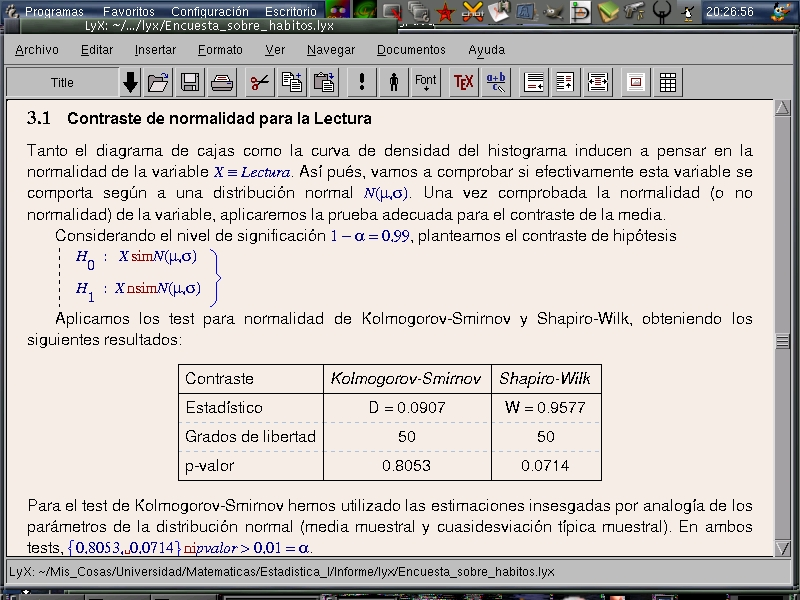
\includegraphics[width=\textwidth]{imagenes/lyx.eps}
\caption{\LyX~ con un trabajo acad�mico sobre inferencia estad�stica}
\end{figure}

